\documentclass[12pt]{article}
\usepackage{geometry}
\geometry{a4paper, margin=1in}
\usepackage{graphicx}
\usepackage{titlesec}
\usepackage{xcolor}
\usepackage{hyperref}
\usepackage{fancyhdr}
\usepackage{enumitem}

% Formatting
\titleformat{\section}{\large\bfseries}{\thesection.}{0.5em}{}
\pagestyle{fancy}
\setlength{\headheight}{15pt}
\fancyhf{}
\rhead{EE175A/B – Weekly Progress Report}
\lhead{Battery Management and Communication System}
\rfoot{Page \thepage}

\begin{document}

\begin{center}
    {\Large \textbf{Weekly Progress Report (WPR)}} \\[6pt]
    {\large \textbf{Battery Management and Communication System (BMS)}} \\[2pt]
    \rule{0.8\textwidth}{0.5pt} \\[6pt]
\end{center}

\noindent
\textbf{Team:} Kaushik Vada, Sachin Patel, Kevin Tran \\[3pt]
\textbf{Course:} EE175A – Senior Design I \\
\textbf{Instructor:} Prof. Sheldon Tan \\
\textbf{Week:}(\textit{Oct 20 – Oct 26, 2025}) \\[8pt]

\vspace{1em}

\section{Work Completed This Week}

\begin{itemize}[leftmargin=1cm]
    \item Focused solely on CAD design and optimization of the BMS enclosure, including mechanical layout and airflow considerations.
\end{itemize}

\vspace{1em}

\section{Challenges Encountered}
\begin{itemize}[leftmargin=1cm]
    \item Limited clearance above the battery pack for PCB and lid integration — required tray redesign and low-profile connectors.
    \item Need to balance airflow for both pack cooling and electronic zone ventilation.
    \item Routing high-voltage sense lines while maintaining isolation distances between battery and STM32 domain.
\end{itemize}

\vspace{1em}

\section{Work Plan for Next Week}
\begin{itemize}[leftmargin=1cm]
    \item Begin STM32 firmware development focusing on USB communication, fan control, and ADC data acquisition.
\end{itemize}

\vspace{1em}

\section{Appendix A – System Block Diagram}
\begin{center}
    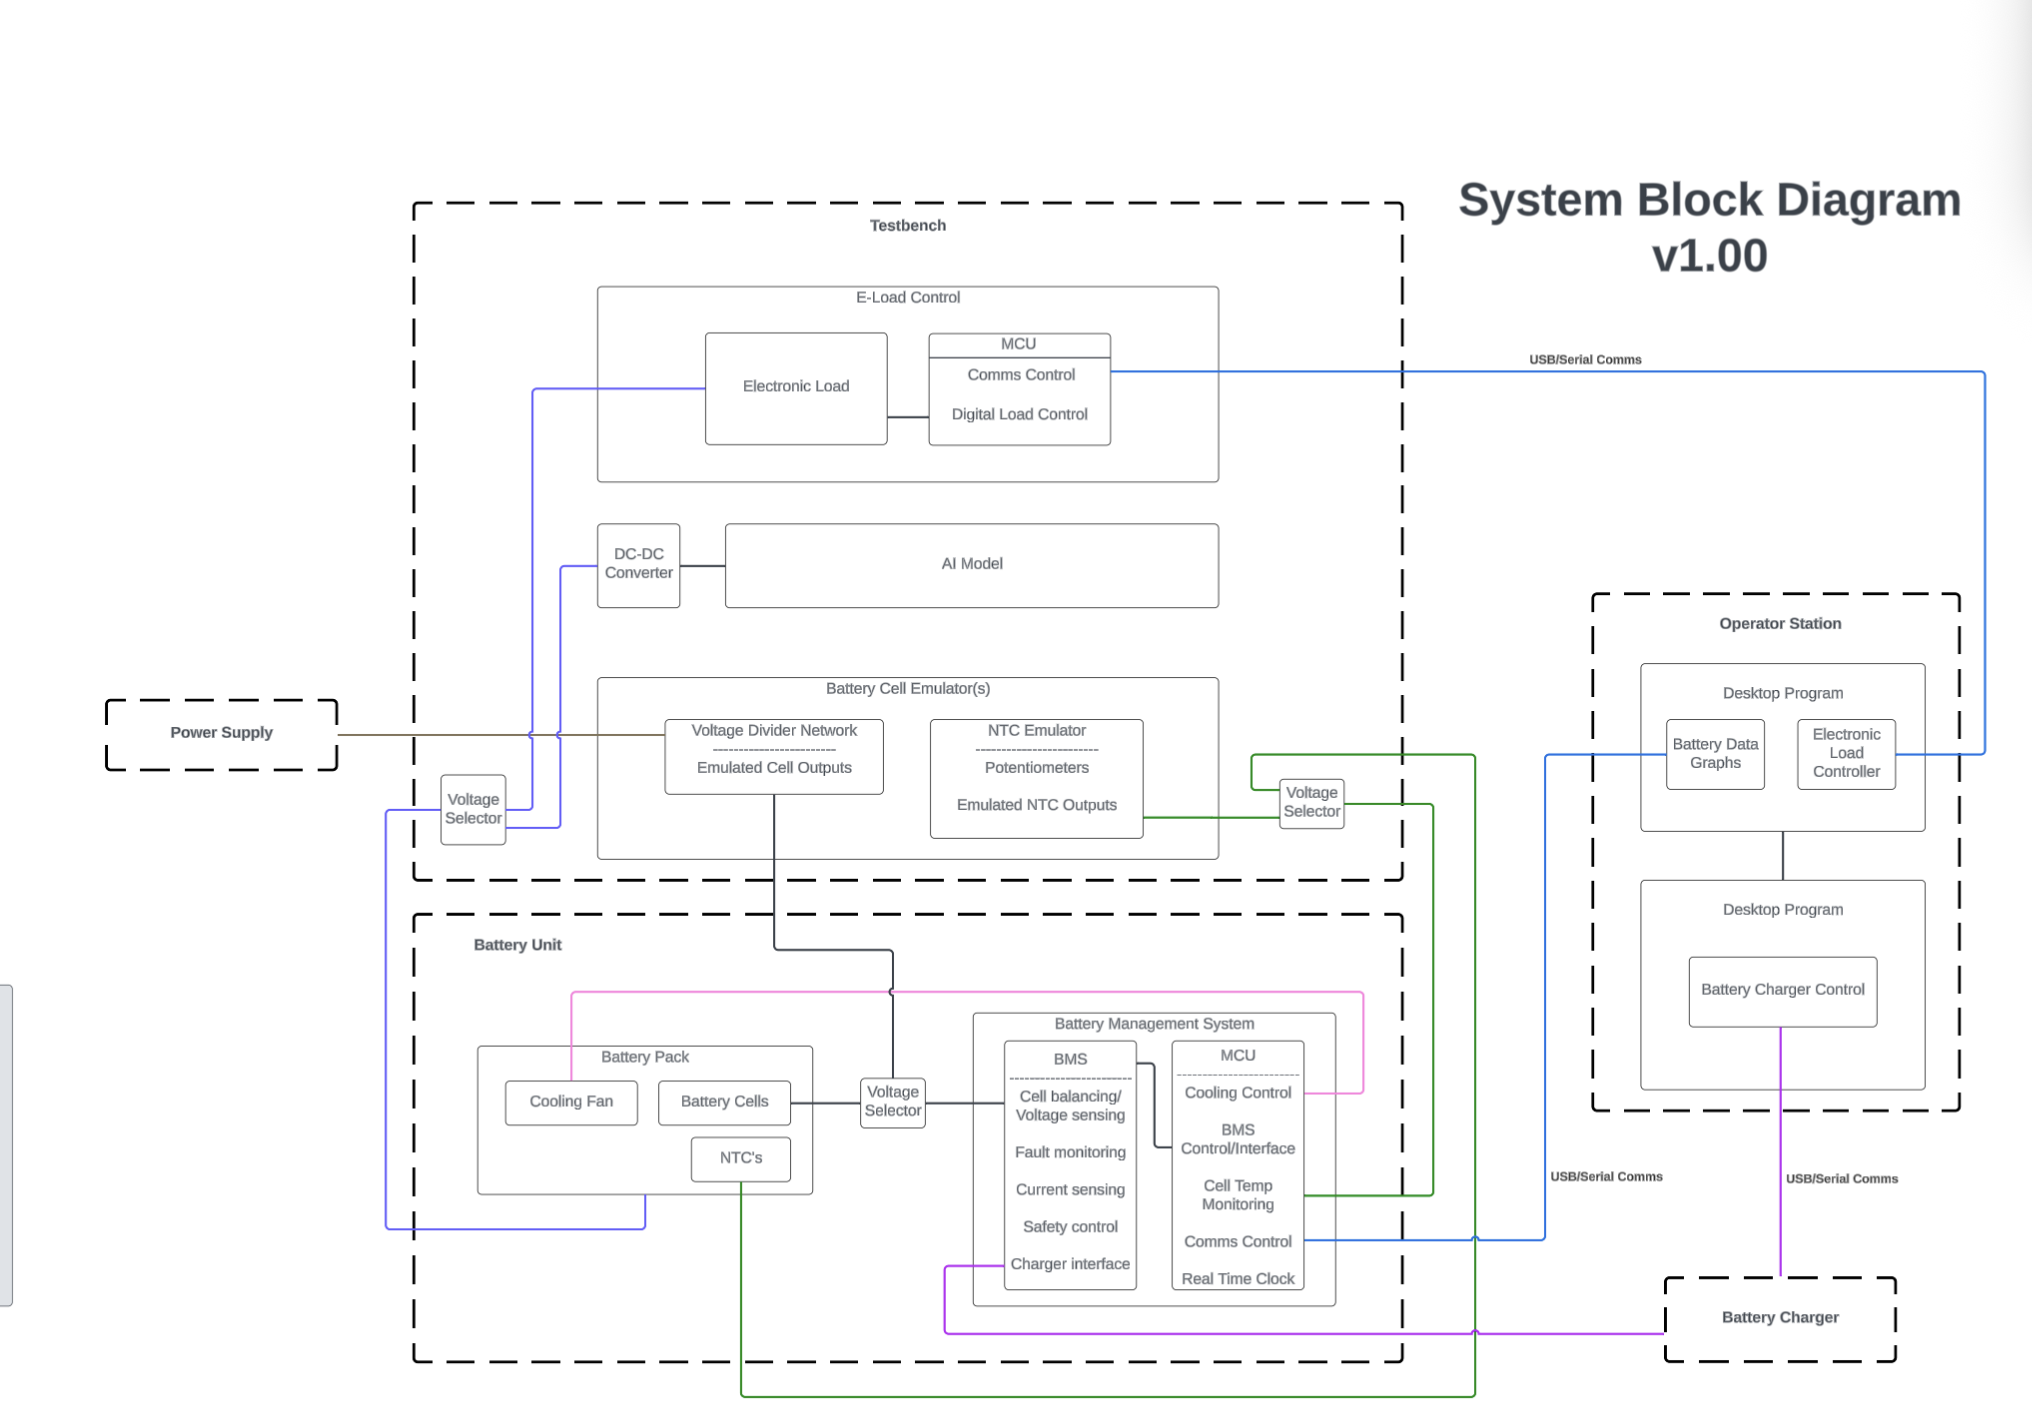
\includegraphics[width=0.95\textwidth]{bms_block_diagram.png} [Figure 1]
\end{center}
\noindent
\textit{Figure A1:} Updated System Block Diagram showing battery domain, isolation components, STM32 communication, and host interface (Source: EE175 Project Report).

\vspace{1em}

\section{Appendix B – Enclosure Visualization}
\begin{center}
    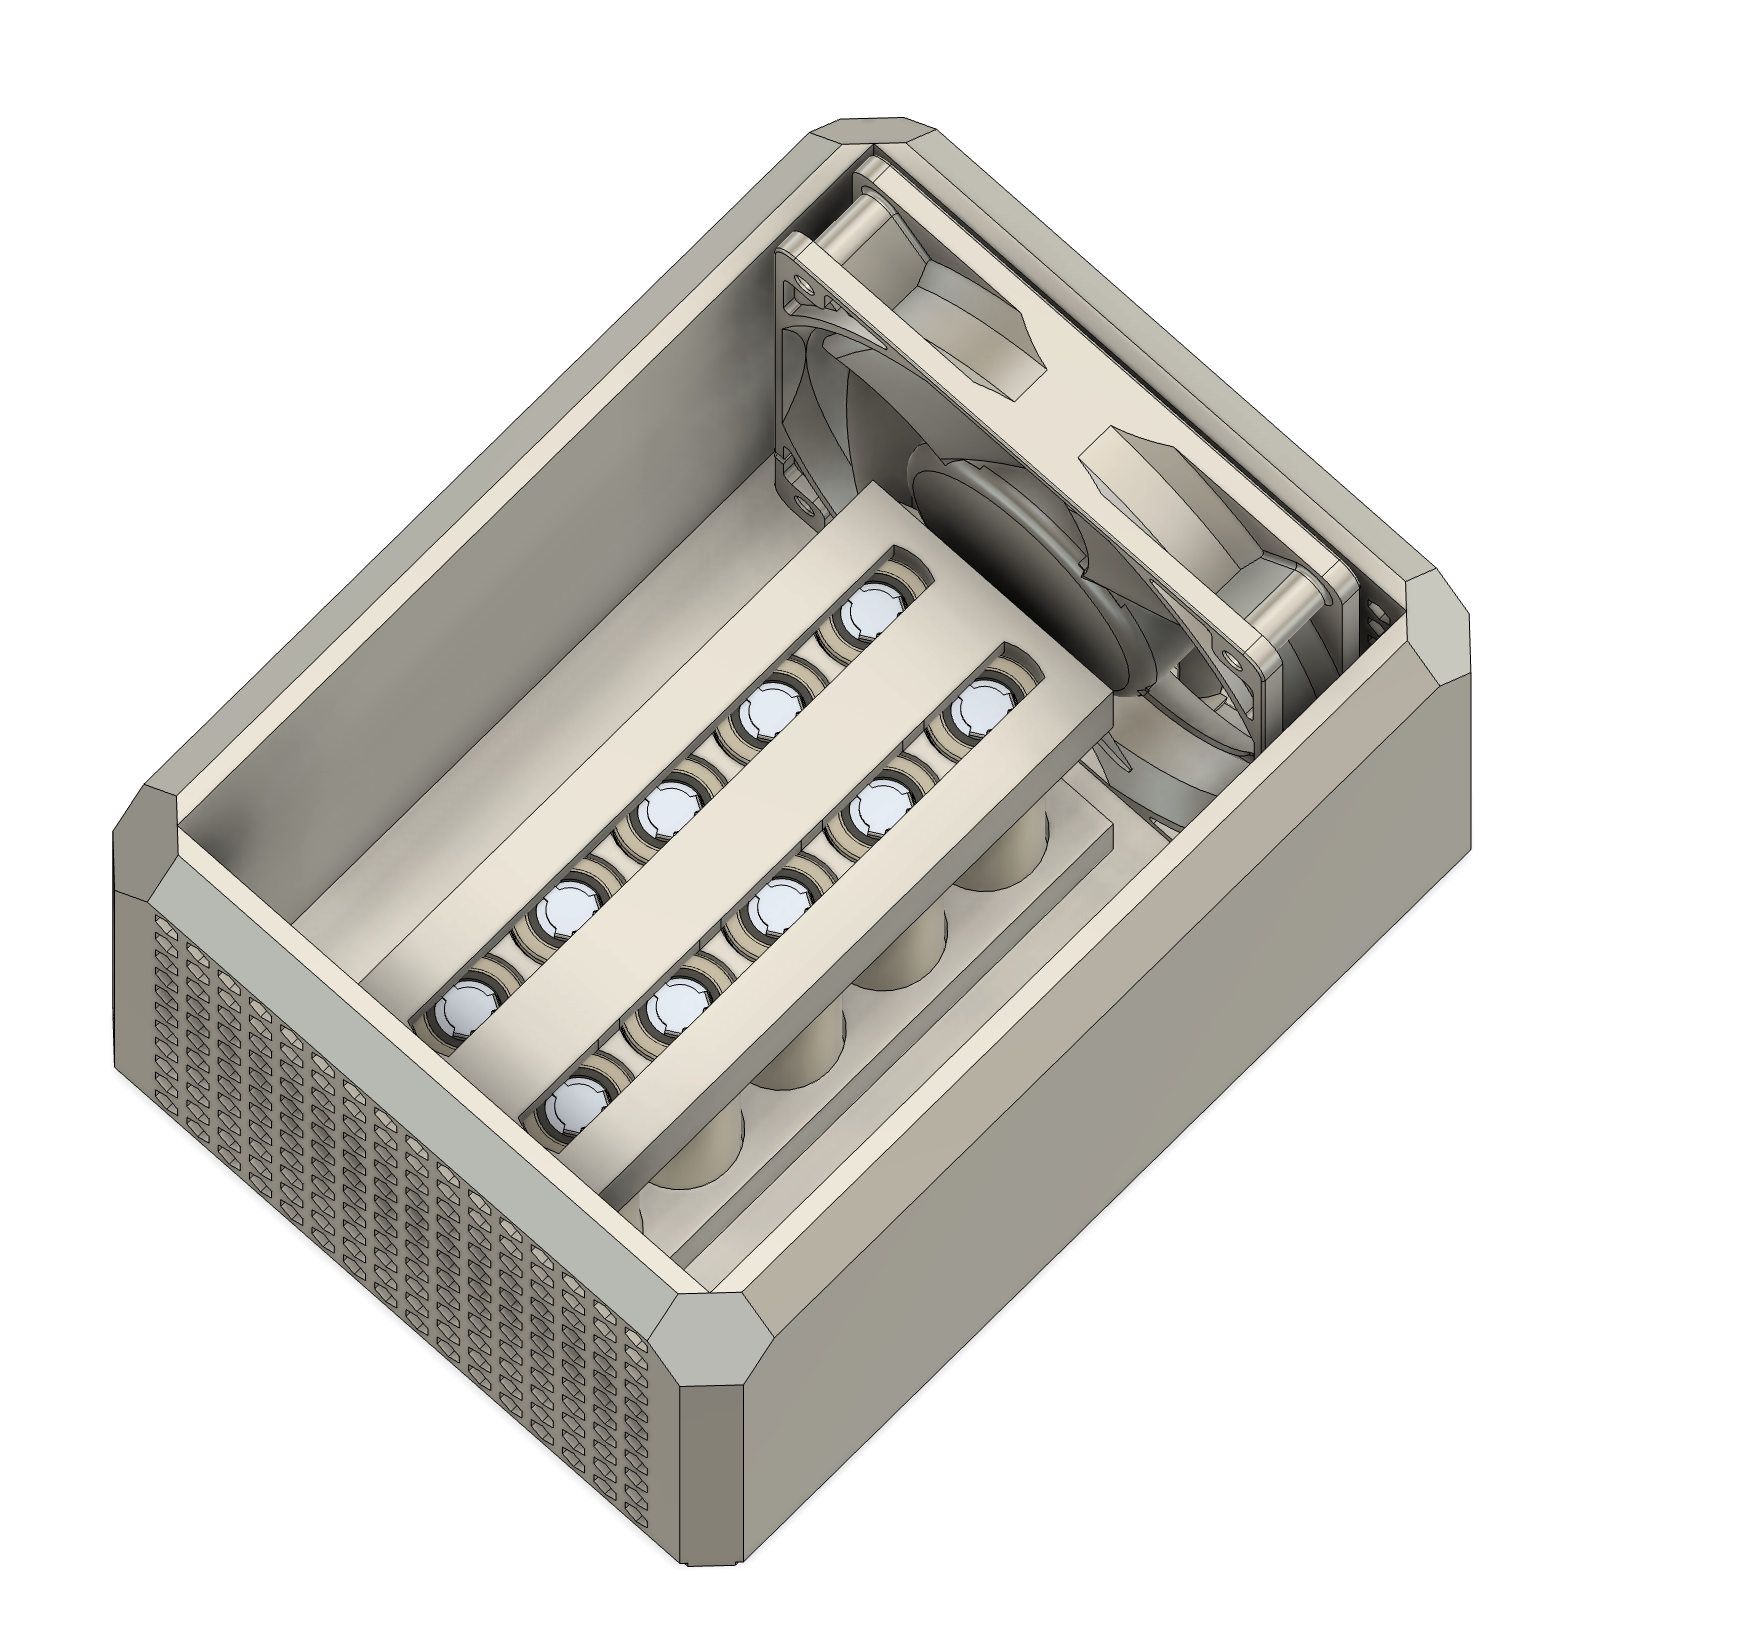
\includegraphics[width=0.95\textwidth]{bms_enclosure_render.png} [Figure 2]
\end{center}
\noindent
\textit{Figure B1:} 3D rendering of BMS enclosure with semi-transparent lid, showing airflow, fan, USB-C port, and internal component placement.

\vspace{1em}

\end{document}